\setAuthor{Eero Vaher}
\setRound{piirkonnavoor}
\setYear{2017}
\setNumber{G 5}
\setDifficulty{4}
\setTopic{Geomeetriline optika}

\prob{Puuduv lääts}
Esemelt lähtuv valgus läbib esmalt nõgusläätse ning seejärel kumerläätse. Joonisel on kujutatud eseme, kumerläätse ning lõpuks tekkiva kujutise asukohad ning kumerläätse fookused $F_k$. Konstrueerige lisalehel nõgusläätse ning selle esemepoolse fookuse $F_n$ asukohad. 

\begin{resizebox}{\linewidth}{!}{
		\begin{tikzpicture}
		\pgfmathsetmacro{\fk}{2}
		\pgfmathsetmacro{\tk}{3*\fk}
		\pgfmathsetmacro{\nk}{1/(1/\fk-1/\tk)}
		\pgfmathsetmacro{\a}{2*\fk}
		\pgfmathsetmacro{\h}{0.5}
		\pgfmathsetmacro{\htk}{\tk/\nk*\h}
		\pgfmathsetmacro{\ha}{1.5*\h}
		\pgfmathsetmacro{\nl}{\nk-\h/(\h-\ha)*(\nk-\a)}
		\pgfmathsetmacro{\fn}{\nk-\h/(\h-\ha)*(\nk-\nl)}
		\coordinate (TK) at (\tk, -\htk);
		\coordinate (NK) at (-\nk, \h);
		\coordinate (A) at (-\a, \ha);
		\draw (-1.1*\fn, 0) -- (1.1*\tk, 0);
		\draw[<->, ultra thick] (0,3.5*\h) -- (0,-3.5*\h);
		\draw[->, ultra thick] (\tk, 0) -- (TK);
		\draw[fill] (-\fk, 0) circle (0.02*\fk) node[below] {$F_k$};
		\draw[fill] (\fk, 0) circle (0.02*\fk) node[below] {$F_k$};
		\draw[->, ultra thick] (-\a, 0) -- (A);
		\end{tikzpicture}}
\end{resizebox}

\hint
Nõguslääts tekitab esemest näiva kujutise ning kumerlääts tekitab näivast kujutisest tõelise kujutise. Kuna kumerläätse asukoht on teada, saab tagurpidi lähenedes rekonstrueerida näilise kujutise asukoha.

\solu
Nõguslääts tekitab esemest näiva kujutise ning kumerlääts tekitab näivast kujutisest tõelise kujutise. Teades kumerläätse asukohta ja fookuseid ning tõelise kujutise asukohta, on võimalik leida näiva kujutise asukoht (joonisel kujutatud sinisega; kujutatud on kolme kiirt, kuid konstrueerimiseks piisab kahest). Teades eseme ning nõgusläätse tekitatud näiva kujutise asukohti, on läätse asukoha ning selle esemepoolse fookuse leidmine lihtne. 

\begin{resizebox}{\linewidth}{!}{
		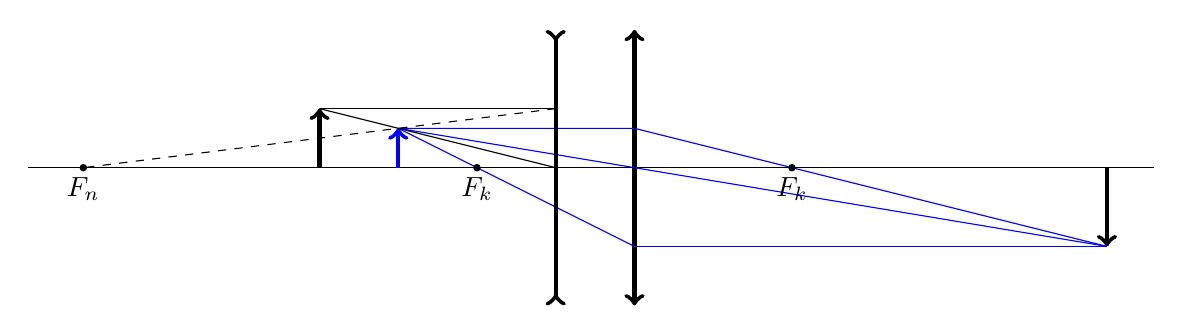
\begin{tikzpicture}
		\pgfmathsetmacro{\fk}{2}
		\pgfmathsetmacro{\tk}{3*\fk}
		\pgfmathsetmacro{\nk}{1/(1/\fk-1/\tk)}
		\pgfmathsetmacro{\a}{2*\fk}
		\pgfmathsetmacro{\h}{0.5}
		\pgfmathsetmacro{\htk}{\tk/\nk*\h}
		\pgfmathsetmacro{\ha}{1.5*\h}
		\pgfmathsetmacro{\nl}{\nk-\h/(\h-\ha)*(\nk-\a)}
		\pgfmathsetmacro{\fn}{\nk-\h/(\h-\ha)*(\nk-\nl)}
		\coordinate (TK) at (\tk, -\htk);
		\coordinate (NK) at (-\nk, \h);
		\coordinate (A) at (-\a, \ha);
		\draw (-1.1*\fn, 0) -- (1.1*\tk, 0);
		\draw[<->, ultra thick] (0,3.5*\h) -- (0,-3.5*\h);
		\draw[->, ultra thick] (\tk, 0) -- (TK);
		\draw[->, ultra thick, blue] (-\nk, 0) -- (NK);
		\draw[blue] (TK) -- (NK);
		\draw[blue] (TK) -- (0,-\htk);
		\draw[blue] (0,-\htk) -- (NK);
		\draw[blue] (TK) -- (0,\h) -- (NK);
		\draw[fill] (-\fk, 0) circle (0.02*\fk) node[below] {$F_k$};
		\draw[fill] (\fk, 0) circle (0.02*\fk) node[below] {$F_k$};
		\draw[->, ultra thick] (-\a, 0) -- (A);
		\draw[>-<, ultra thick] (-\nl, 3.5*\h) -- (-\nl, -3.5*\h);
		\draw (-\nl, 0) -- (A) -- (NK);
		\draw (A) -- (-\nl, \ha);
		\draw[dashed] (-\nl, \ha) -- (-\fn,0);
		\draw[fill] (-\fn, 0) circle (0.02*\fk) node[below] {$F_n$};
		\end{tikzpicture}}
\end{resizebox}

\probeng{Missing lens}
A light originating from an object first goes through a concave lens and then a convex lens. The locations of the object, the convex lens and the forming image are shown in the figure, the focal points $F_k$ of the convex lens are also included. Construct the locations of the concave lens and the focal point $F_n$ that is closer to the object.\\
\begin{resizebox}{\linewidth}{!}{
		\begin{tikzpicture}
		\pgfmathsetmacro{\fk}{2}
		\pgfmathsetmacro{\tk}{3*\fk}
		\pgfmathsetmacro{\nk}{1/(1/\fk-1/\tk)}
		\pgfmathsetmacro{\a}{2*\fk}
		\pgfmathsetmacro{\h}{0.5}
		\pgfmathsetmacro{\htk}{\tk/\nk*\h}
		\pgfmathsetmacro{\ha}{1.5*\h}
		\pgfmathsetmacro{\nl}{\nk-\h/(\h-\ha)*(\nk-\a)}
		\pgfmathsetmacro{\fn}{\nk-\h/(\h-\ha)*(\nk-\nl)}
		\coordinate (TK) at (\tk, -\htk);
		\coordinate (NK) at (-\nk, \h);
		\coordinate (A) at (-\a, \ha);
		\draw (-1.1*\fn, 0) -- (1.1*\tk, 0);
		\draw[<->, ultra thick] (0,3.5*\h) -- (0,-3.5*\h);
		\draw[->, ultra thick] (\tk, 0) -- (TK);
		\draw[fill] (-\fk, 0) circle (0.02*\fk) node[below] {$F_k$};
		\draw[fill] (\fk, 0) circle (0.02*\fk) node[below] {$F_k$};
		\draw[->, ultra thick] (-\a, 0) -- (A);
		\end{tikzpicture}}
\end{resizebox}

\hinteng
The concave lens makes a virtual image of the object and the convex lens makes a real image of the virtual image. Since the location of the convex lens is known you can find the location of the virtual image by reconstructing with a backwards approach.

\solueng
The concave lens creates a virtual image of the object and the convex lens creates a real image of the virtual image. Knowing the location and focal points of the convex lens and the location of the real image it is possible to find the location of the virtual image (in the image it is depicted with blue; three rays are pictured but for constructing two will suffice). Knowing the locations of the object and the virtual image created by the concave lens it is easy to find the location of the lens and its focal point that is on the same side as the object.\\
\begin{resizebox}{\linewidth}{!}{
		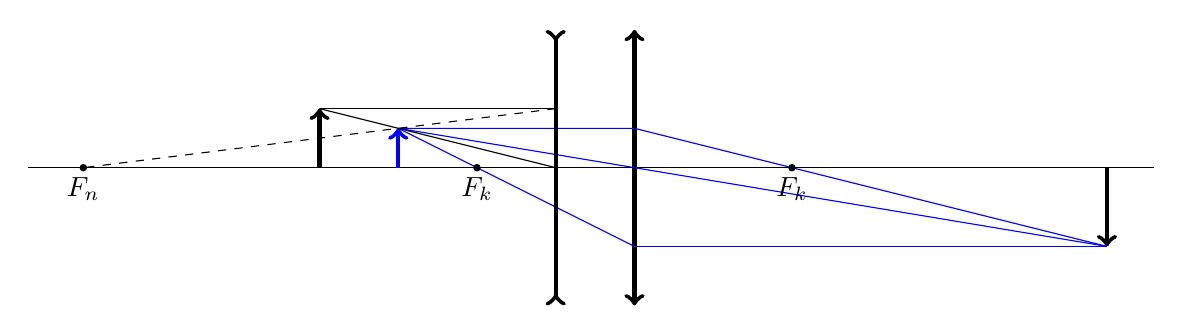
\begin{tikzpicture}
		\pgfmathsetmacro{\fk}{2}
		\pgfmathsetmacro{\tk}{3*\fk}
		\pgfmathsetmacro{\nk}{1/(1/\fk-1/\tk)}
		\pgfmathsetmacro{\a}{2*\fk}
		\pgfmathsetmacro{\h}{0.5}
		\pgfmathsetmacro{\htk}{\tk/\nk*\h}
		\pgfmathsetmacro{\ha}{1.5*\h}
		\pgfmathsetmacro{\nl}{\nk-\h/(\h-\ha)*(\nk-\a)}
		\pgfmathsetmacro{\fn}{\nk-\h/(\h-\ha)*(\nk-\nl)}
		\coordinate (TK) at (\tk, -\htk);
		\coordinate (NK) at (-\nk, \h);
		\coordinate (A) at (-\a, \ha);
		\draw (-1.1*\fn, 0) -- (1.1*\tk, 0);
		\draw[<->, ultra thick] (0,3.5*\h) -- (0,-3.5*\h);
		\draw[->, ultra thick] (\tk, 0) -- (TK);
		\draw[->, ultra thick, blue] (-\nk, 0) -- (NK);
		\draw[blue] (TK) -- (NK);
		\draw[blue] (TK) -- (0,-\htk);
		\draw[blue] (0,-\htk) -- (NK);
		\draw[blue] (TK) -- (0,\h) -- (NK);
		\draw[fill] (-\fk, 0) circle (0.02*\fk) node[below] {$F_k$};
		\draw[fill] (\fk, 0) circle (0.02*\fk) node[below] {$F_k$};
		\draw[->, ultra thick] (-\a, 0) -- (A);
		\draw[>-<, ultra thick] (-\nl, 3.5*\h) -- (-\nl, -3.5*\h);
		\draw (-\nl, 0) -- (A) -- (NK);
		\draw (A) -- (-\nl, \ha);
		\draw[dashed] (-\nl, \ha) -- (-\fn,0);
		\draw[fill] (-\fn, 0) circle (0.02*\fk) node[below] {$F_n$};
		\end{tikzpicture}}
\end{resizebox}
\probend